% Options for packages loaded elsewhere
\PassOptionsToPackage{unicode}{hyperref}
\PassOptionsToPackage{hyphens}{url}
%
\documentclass[
]{article}
\usepackage{amsmath,amssymb}
\usepackage{lmodern}
\usepackage{ifxetex,ifluatex}
\ifnum 0\ifxetex 1\fi\ifluatex 1\fi=0 % if pdftex
  \usepackage[T1]{fontenc}
  \usepackage[utf8]{inputenc}
  \usepackage{textcomp} % provide euro and other symbols
\else % if luatex or xetex
  \usepackage{unicode-math}
  \defaultfontfeatures{Scale=MatchLowercase}
  \defaultfontfeatures[\rmfamily]{Ligatures=TeX,Scale=1}
\fi
% Use upquote if available, for straight quotes in verbatim environments
\IfFileExists{upquote.sty}{\usepackage{upquote}}{}
\IfFileExists{microtype.sty}{% use microtype if available
  \usepackage[]{microtype}
  \UseMicrotypeSet[protrusion]{basicmath} % disable protrusion for tt fonts
}{}
\makeatletter
\@ifundefined{KOMAClassName}{% if non-KOMA class
  \IfFileExists{parskip.sty}{%
    \usepackage{parskip}
  }{% else
    \setlength{\parindent}{0pt}
    \setlength{\parskip}{6pt plus 2pt minus 1pt}}
}{% if KOMA class
  \KOMAoptions{parskip=half}}
\makeatother
\usepackage{xcolor}
\IfFileExists{xurl.sty}{\usepackage{xurl}}{} % add URL line breaks if available
\IfFileExists{bookmark.sty}{\usepackage{bookmark}}{\usepackage{hyperref}}
\hypersetup{
  pdftitle={PhyCovA Tutorial},
  hidelinks,
  pdfcreator={LaTeX via pandoc}}
\urlstyle{same} % disable monospaced font for URLs
\usepackage[margin=1in]{geometry}
\usepackage{graphicx}
\makeatletter
\def\maxwidth{\ifdim\Gin@nat@width>\linewidth\linewidth\else\Gin@nat@width\fi}
\def\maxheight{\ifdim\Gin@nat@height>\textheight\textheight\else\Gin@nat@height\fi}
\makeatother
% Scale images if necessary, so that they will not overflow the page
% margins by default, and it is still possible to overwrite the defaults
% using explicit options in \includegraphics[width, height, ...]{}
\setkeys{Gin}{width=\maxwidth,height=\maxheight,keepaspectratio}
% Set default figure placement to htbp
\makeatletter
\def\fps@figure{htbp}
\makeatother
\setlength{\emergencystretch}{3em} % prevent overfull lines
\providecommand{\tightlist}{%
  \setlength{\itemsep}{0pt}\setlength{\parskip}{0pt}}
\setcounter{secnumdepth}{5}
\ifluatex
  \usepackage{selnolig}  % disable illegal ligatures
\fi

\title{PhyCovA Tutorial}
\author{}
\date{\vspace{-2.5em}08/02/2022}

\begin{document}
\maketitle

{
\setcounter{tocdepth}{3}
\tableofcontents
}
\hypertarget{getting-started}{%
\section{Getting started}\label{getting-started}}

\hypertarget{browser-based-app}{%
\subsection{Browser-based app}\label{browser-based-app}}

There are 2 ways on how to get started with PhyCovA. The first being via
the browser and opening the following web-page:
\url{https://evolcompvir-kuleuven.shinyapps.io/PhyCovA/}

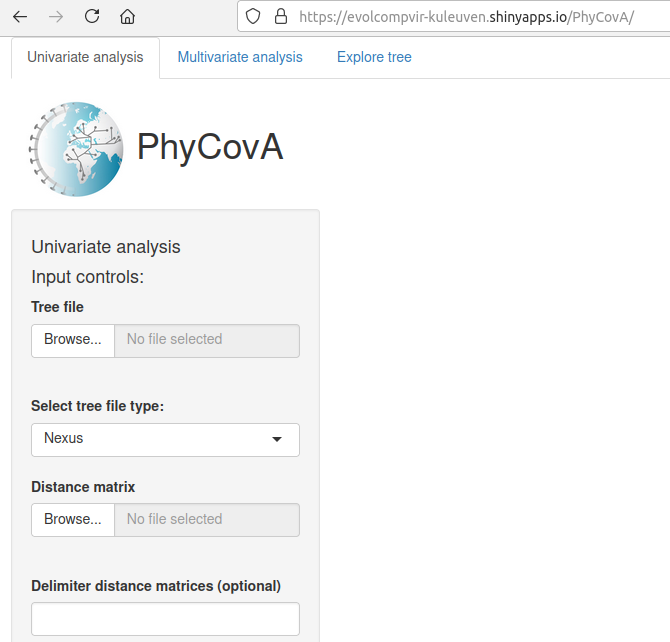
\includegraphics{tutorial_img/evolcompvir_start_up.png}

\hypertarget{docker-image}{%
\subsection{Docker image}\label{docker-image}}

The 2nd method is to download (``pull'') the docker image available on
dockerhub. Installing docker will not be part of this tutorial but good
tutorials are available from:
\url{https://docs.docker.com/engine/install/}

\url{https://docs.docker.com/engine/install/ubuntu/}

Once the docker engine is correctly installed we can proceed with
pulling the image for PhyCovA. First a few words on docker terminology.
The normal docker workflow is:

\textbf{Dockerfile -\textgreater{} Image -\textgreater{} Container}

The dockerfile contains the instructions that the docker engine needs to
``build'' the image. The docker image is ``frozen'' and contains
everything the docker needs to work. An operating system, R, the
required packages, python and the TreeTime package.

The first step is to pull the image from dockerhub:
\url{https://hub.docker.com/repository/docker/timblokker/phycova} :

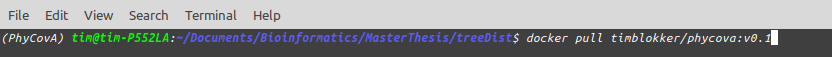
\includegraphics{tutorial_img/Pull_Docker.png}

Pay attention to the ``tag'' of the docker image, which is the text
behind the ``:''. For newer versions of PhyCovA, surf to the dockerhub
repository and check which versions are available, by specifying the
tag/version in the ``pull'' command you obtain the required version.

\textbf{\texttt{docker\ pull\ timblokker/PhyCovA:v0.1}}

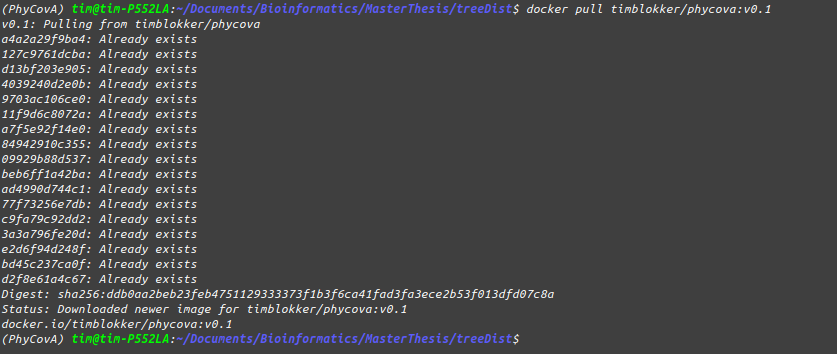
\includegraphics{tutorial_img/Pulled_Docker.png}

Next the docker image is available on your machine, you can check this
by running:

\textbf{\texttt{docker\ images}}

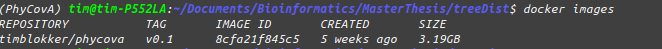
\includegraphics{tutorial_img/Docker_Images.png}

And with this we can proceed to starting the container from the image we
pulled:

\textbf{\texttt{docker\ run\ -d\ -p\ 3838:3838\ timblokker/phycova:v0.1}}

It is possible to run the docker without the ``-d''\emph{etached} flag
to still see the output which when running the shiny app from within
RStudio is outputted on the RStudio console.The ``-p''\emph{ort} flag
specifies the port that will be allocated to PhyCovA. This needs to be
3838 and is hard-coded in the Dockerfile.

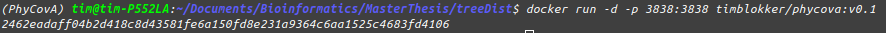
\includegraphics{tutorial_img/Docker_Run.png}

Finally, the browser can be pointed to \url{http://localhost:3838/}

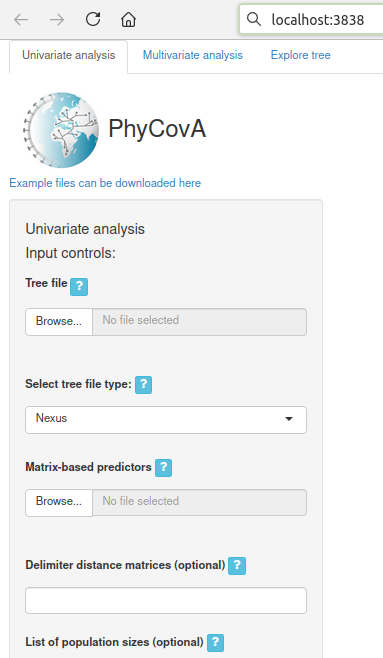
\includegraphics{tutorial_img/Docker_Started.png}

\hypertarget{phycova}{%
\section{PhyCovA}\label{phycova}}

PhyCovA can correlate transition counts or rates obtained from either
trees already annotated with ancestral state information or reconstruct
and annotate the ancestral states before correlating the variables.

In this tutorial data originally published in the publication below will
be examplary analyzed.

Dudas, G., Carvalho, L. M., Bedford, T., Tatem, A. J., Baele, G., Faria,
N. R., Park, D. J., Ladner, J. T., Arias, A., Asogun, D., Bielejec, F.,
Caddy, S. L., Cotten, M., D'Ambrozio, J., Dellicour, S., Di Caro, A.,
Diclaro, J. W., Duraffour, S., Elmore, M. J., \ldots{} Rambaut, A.
(2017). Virus genomes reveal factors that spread and sustained the Ebola
epidemic. Nature, 544(7650), 309--315.
\url{https://doi.org/10.1038/nature22040}

\hypertarget{already-annotated-trees}{%
\subsection{Already annotated trees}\label{already-annotated-trees}}

\hypertarget{univariate-tab}{%
\subsubsection{Univariate tab}\label{univariate-tab}}

The already annotated mode requires only 2 files, the phylogeny, here we
will use an MCC tree for the ebola data set and at least 1 distance
matrix. The data can be obtained from github:
\url{https://github.com/TimBlokker/PhyCovA/tree/master/input/ebola} .
The annotations in the tree must \textbf{exactly} match the column names
in the pairwise distance matrices. And the phylogeny needs to be rooted.

At first we upload the 2 documents using the file-upload panels, by
clicking \textbf{``Browse\ldots{}''}, this will open a file explorer and
should be intuitive to use. \textbf{Note:} For the distance matrix
multiple files can be selected in the file explorer, while the ``Tree
File'' file upload only allows 1 file.

In the screenshot below the 2 file types were successfully uploaded.
Additional limitations on the files are:

\begin{itemize}
\item
  File names can not start with a digit
\item
  Hyphens (``-'') are not recommended, rather use underscores (``\_'')
\end{itemize}

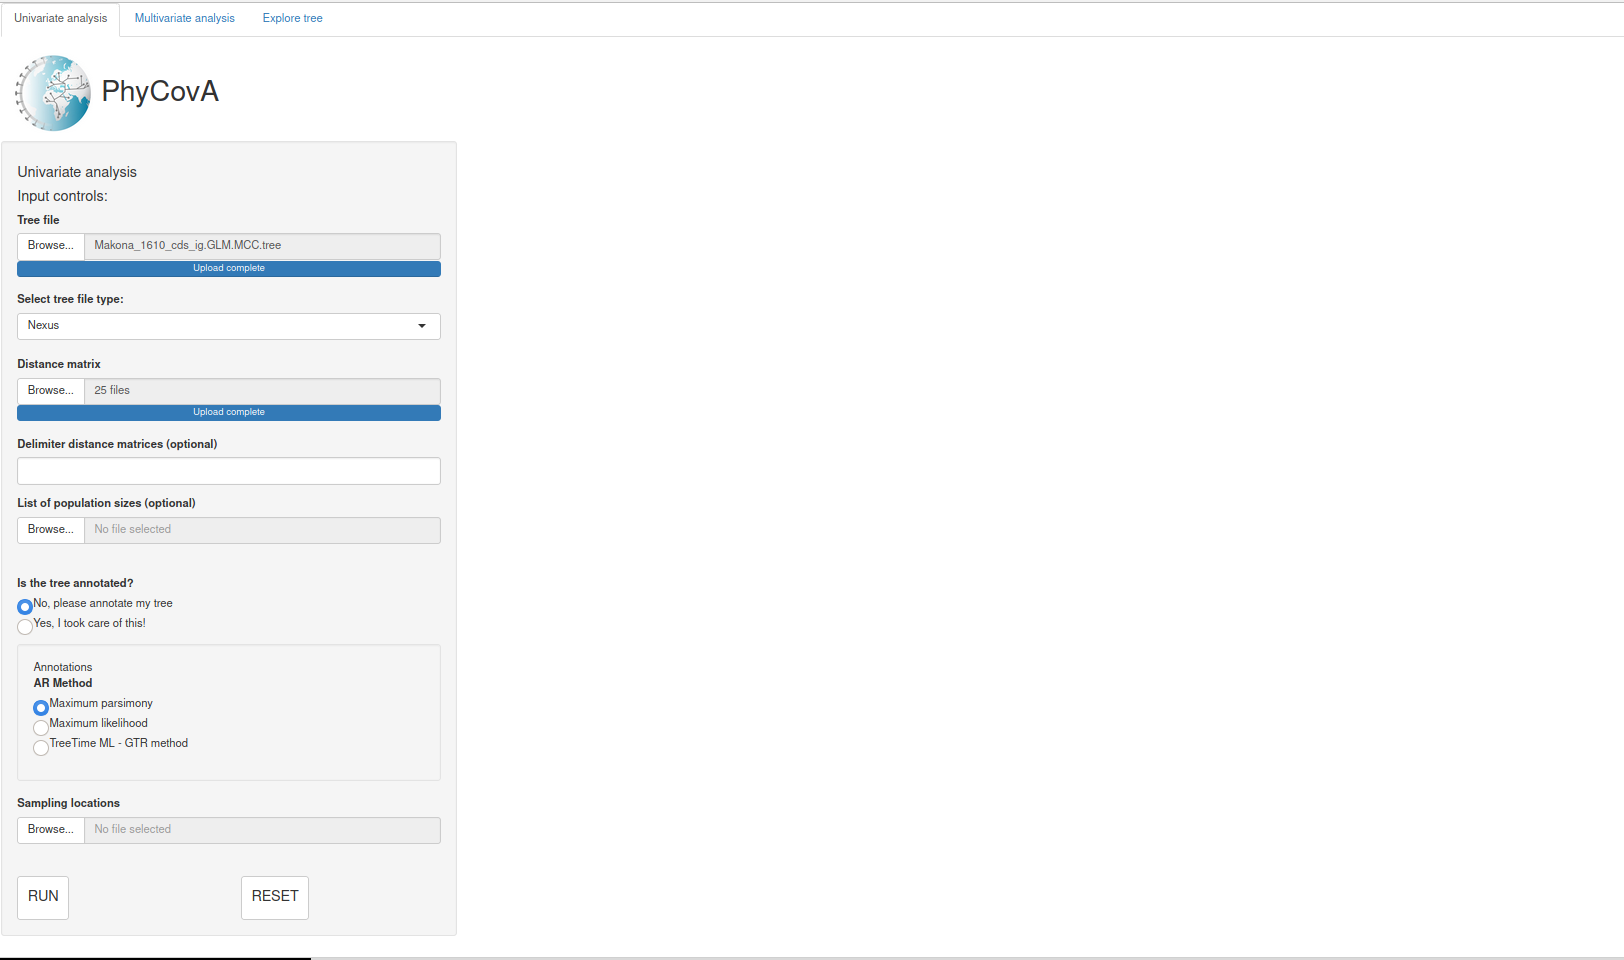
\includegraphics{tutorial_img/Annotated_before_run.png}

When selecting ``Yes, I took care of this!'' then PhyCovA will start
searching for annotations in the tree file that match the column namesof
the distance matrix.

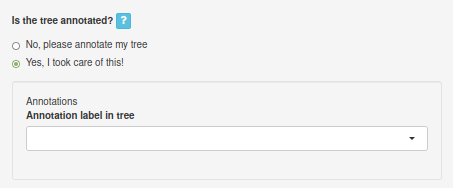
\includegraphics{tutorial_img/Annotation_label_notfoundyet.png}

Once an annotation was found that matches the column names in the
distance matrix, PhyCovA will inform the user.

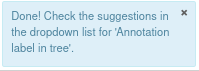
\includegraphics{tutorial_img/Annotation_PopUp.png}

Simultaneously the found column will be displayed. In case more than one
column matches the column names in the matrix the user can select the
appropriate one.

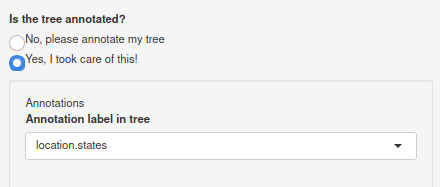
\includegraphics{tutorial_img/SelectedColumn_Found.png}

With this PhyCovA has been given all required information and the
phylogenetic covariance analysis can start by clicking ``RUN''.
Immediately after clicking the input fields will appear but depending on
the size of the tree and the number of distance matrices, the analysis
might take a few seconds to 30 seconds.

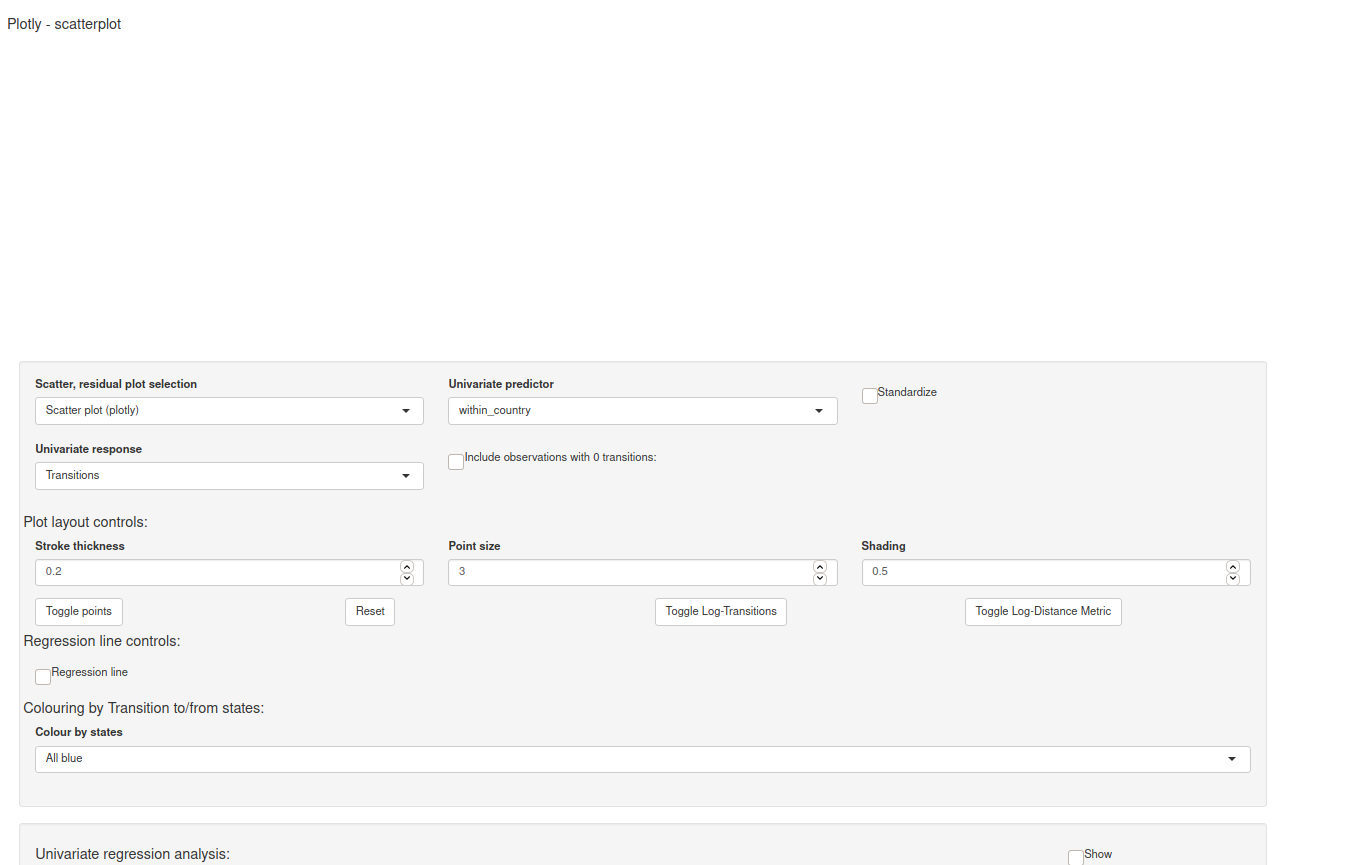
\includegraphics{tutorial_img/Loading_Run.png}

After the covariate analysis has been finished the scatterplot is
visible. At first we see a scatterplot of a binary variable which is not
very informative, so we change the predictor to
``greatCircleDistances''.

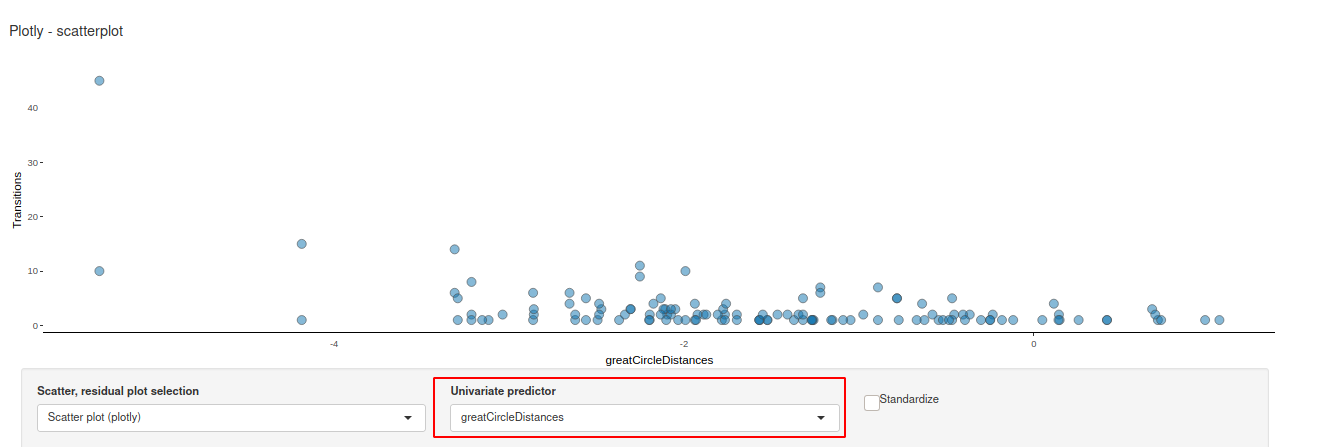
\includegraphics{tutorial_img/changePredictor.png}

There are many options to improve the layout of the plots. We will leave
the user to explore but some important features we would like to point
out. At first the regression line can be drawn in the plot:

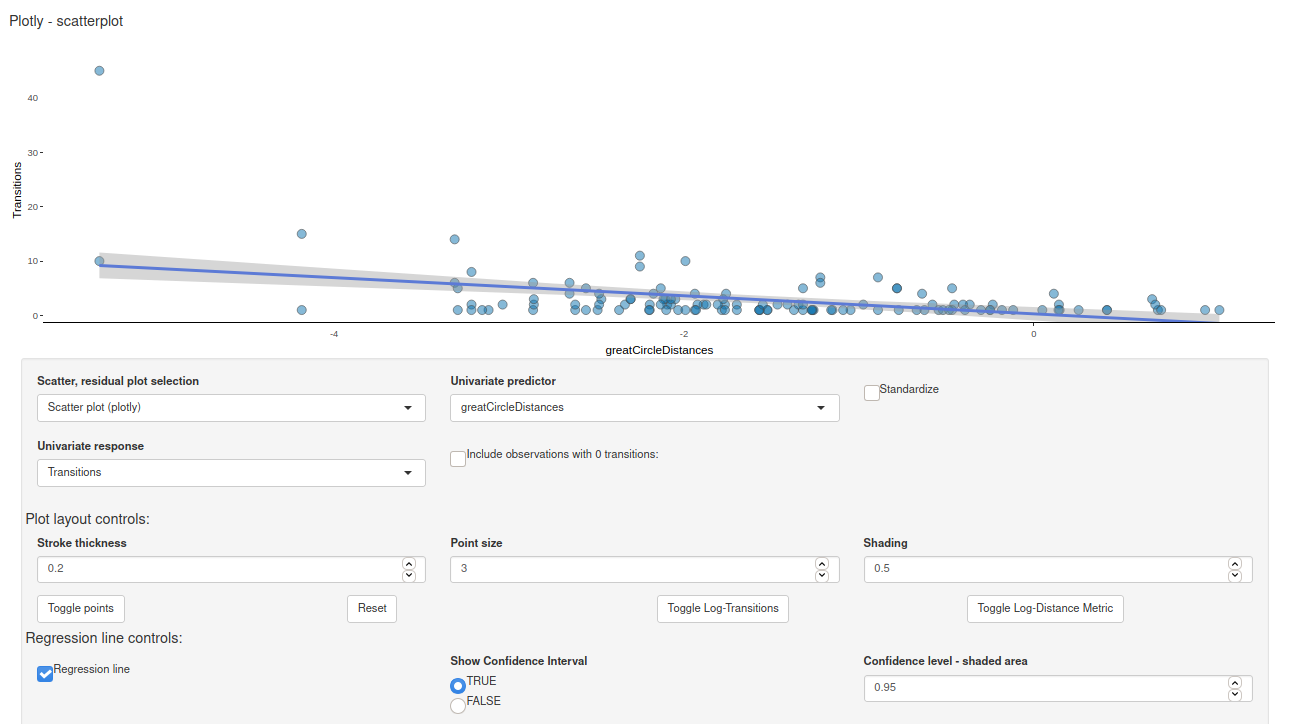
\includegraphics{tutorial_img/Regression_line.png}

Then we can look at the residuals of linear regression:

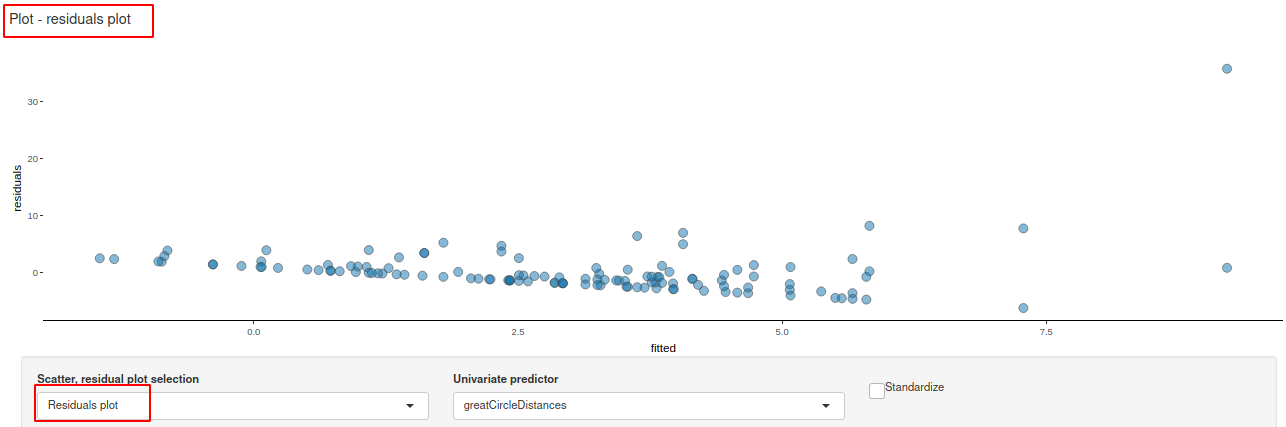
\includegraphics{tutorial_img/Residuals.png}

Observations can be excluded to see which effect particular points have
on the regression. This can be done by brushing points with the ``Box
Select'' tool and then clicking ``Toggle points''. The points are then
removed from the data set used for the regression analysis but are still
plotted in another colour:

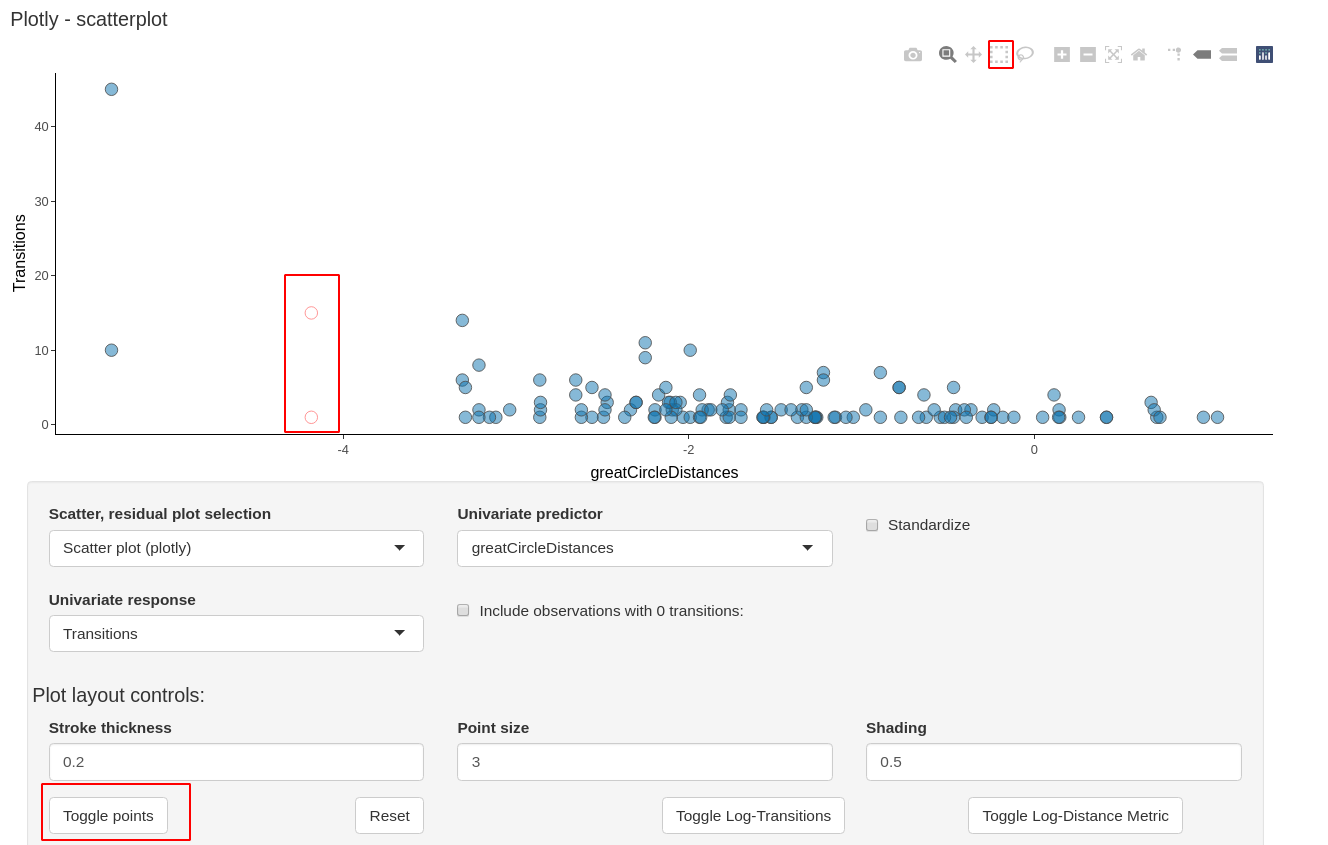
\includegraphics{tutorial_img/toggle_points.png}

The response and the predictor variable can be log-transformed but there
are limitations like the log of 0 and negative values is not defined and
so e.g.~when including zero-transition events the log transformation of
the response variable ``Transition counts'' will not be possible
anymore. Same counts for standardising of the predictors, centering
variables with mean 0 will unavoidably lead to negative values in the
data set.

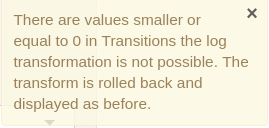
\includegraphics{tutorial_img/WarningLog.png}
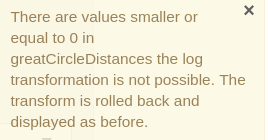
\includegraphics{tutorial_img/Warning.png}

The predictors can be standardized, and zero-transition events can be
included. Zero-transition events are transition events that have not
been observed in the tree. Then the transition events can be colorized
grouped by the origin location (``from'') or also destination (``to'').

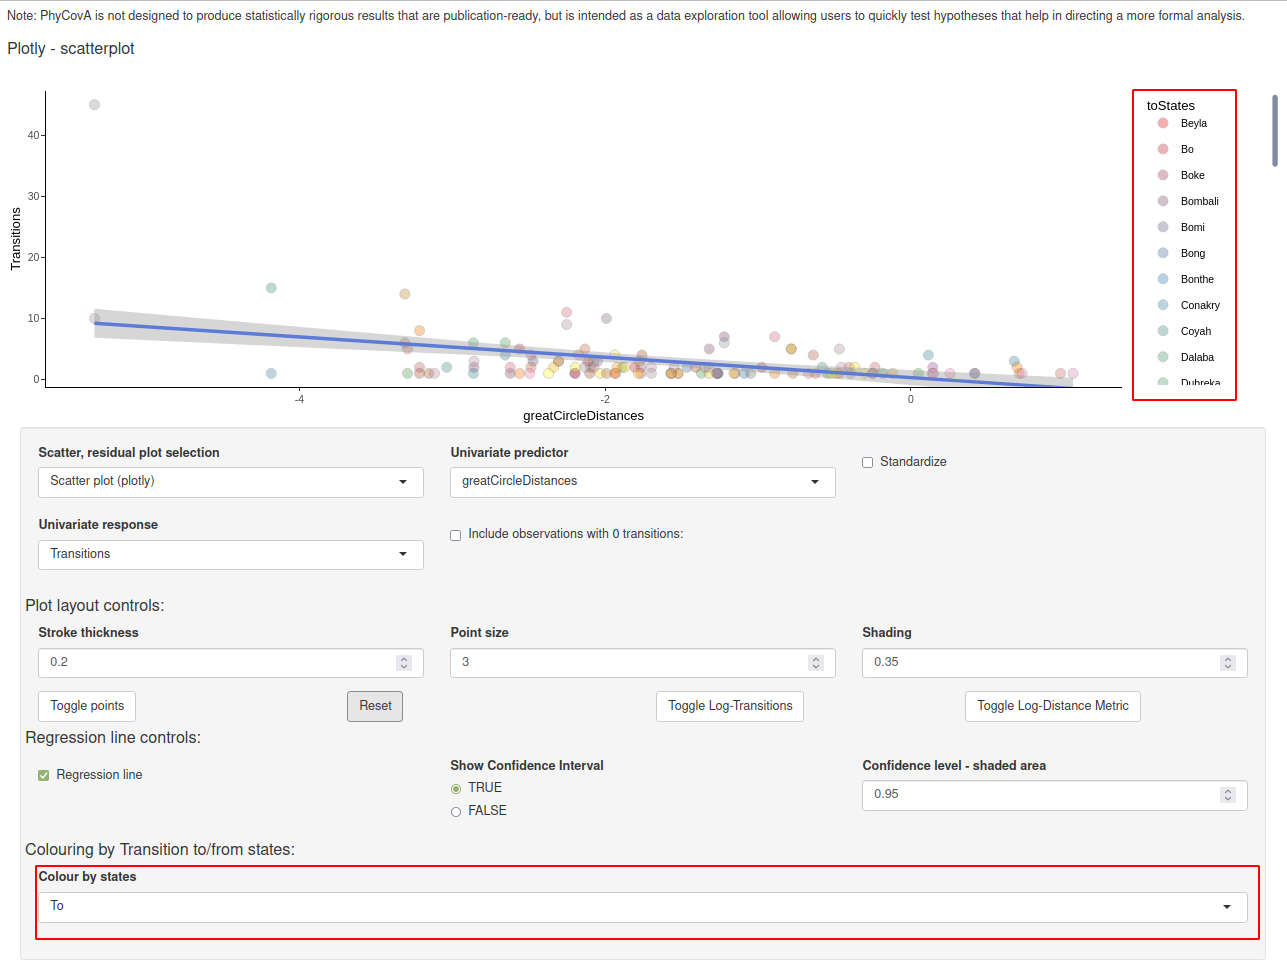
\includegraphics{tutorial_img/colourFrom.png}

Lastly, PhyCovA also offers the option to summarize the transition
counts by state in a bar diagram. Also here we can group observation by
origin country or destination country. The option to include
0-transitions has no effect here (because we add 0\ldots).

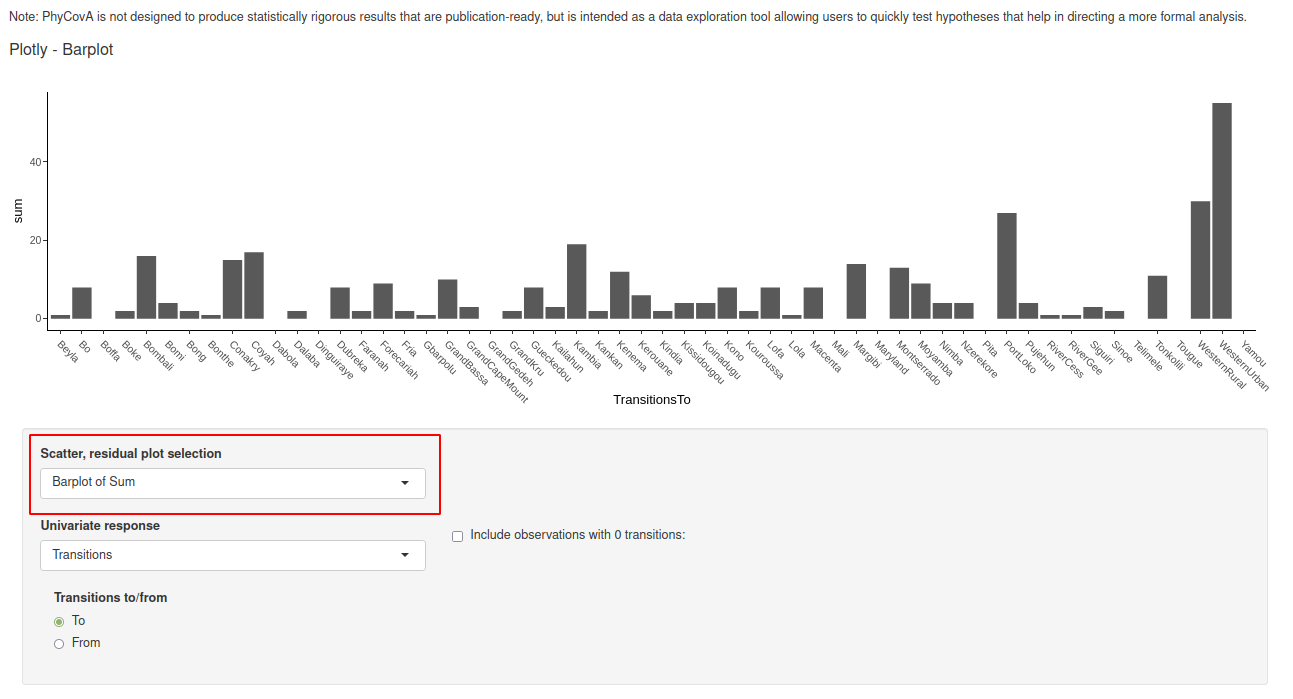
\includegraphics{tutorial_img/UNi_Bar.png}

For this univariate case the standardization and the inclusion of the
0-transitions have impact on the regression output. And this is shown
and updated upon changing the input and is shown as depicted below:

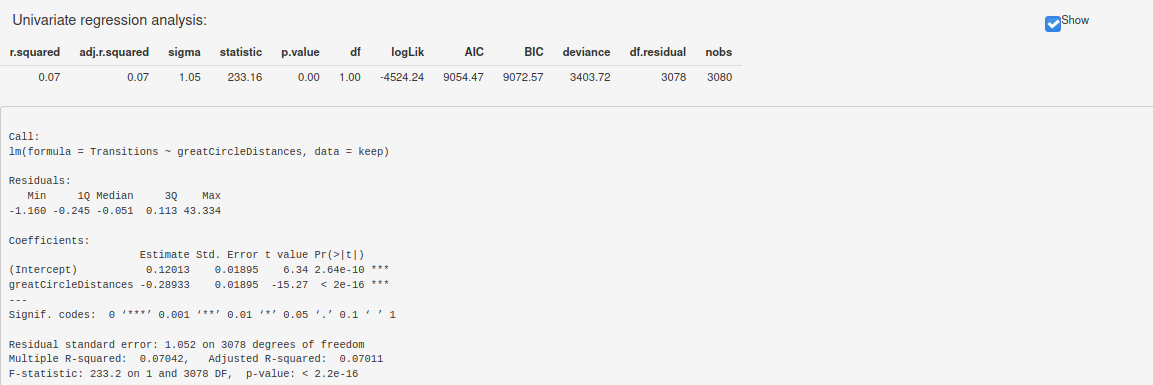
\includegraphics{tutorial_img/Univariate_Regression.png}

From here we can see that the geographic distance (greatCircleDistances)
explains approximately 7\% of the observed transition events (when not
including zero-transitions, not standardizing).

\hypertarget{multivariate-tab}{%
\subsubsection{Multivariate tab}\label{multivariate-tab}}

Switching to the multivariate tab can be done on top of the screen:

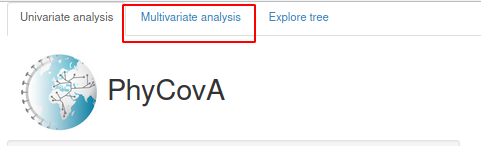
\includegraphics{tutorial_img/Multivariate_tab.png}

On the multivariate tab, at first the variables to include in the
analysis can be selected. We will start with keeping them all selected.
And we will standardize all continuous predictors. We will keep only
actually observed transition events in the data set and will not log
transform the response, for this data set only the ``Transition count''
variable is available as response (drop-down menu in the top left
corner, here for the TreeTime reconstructions also the transition rate
will be available).

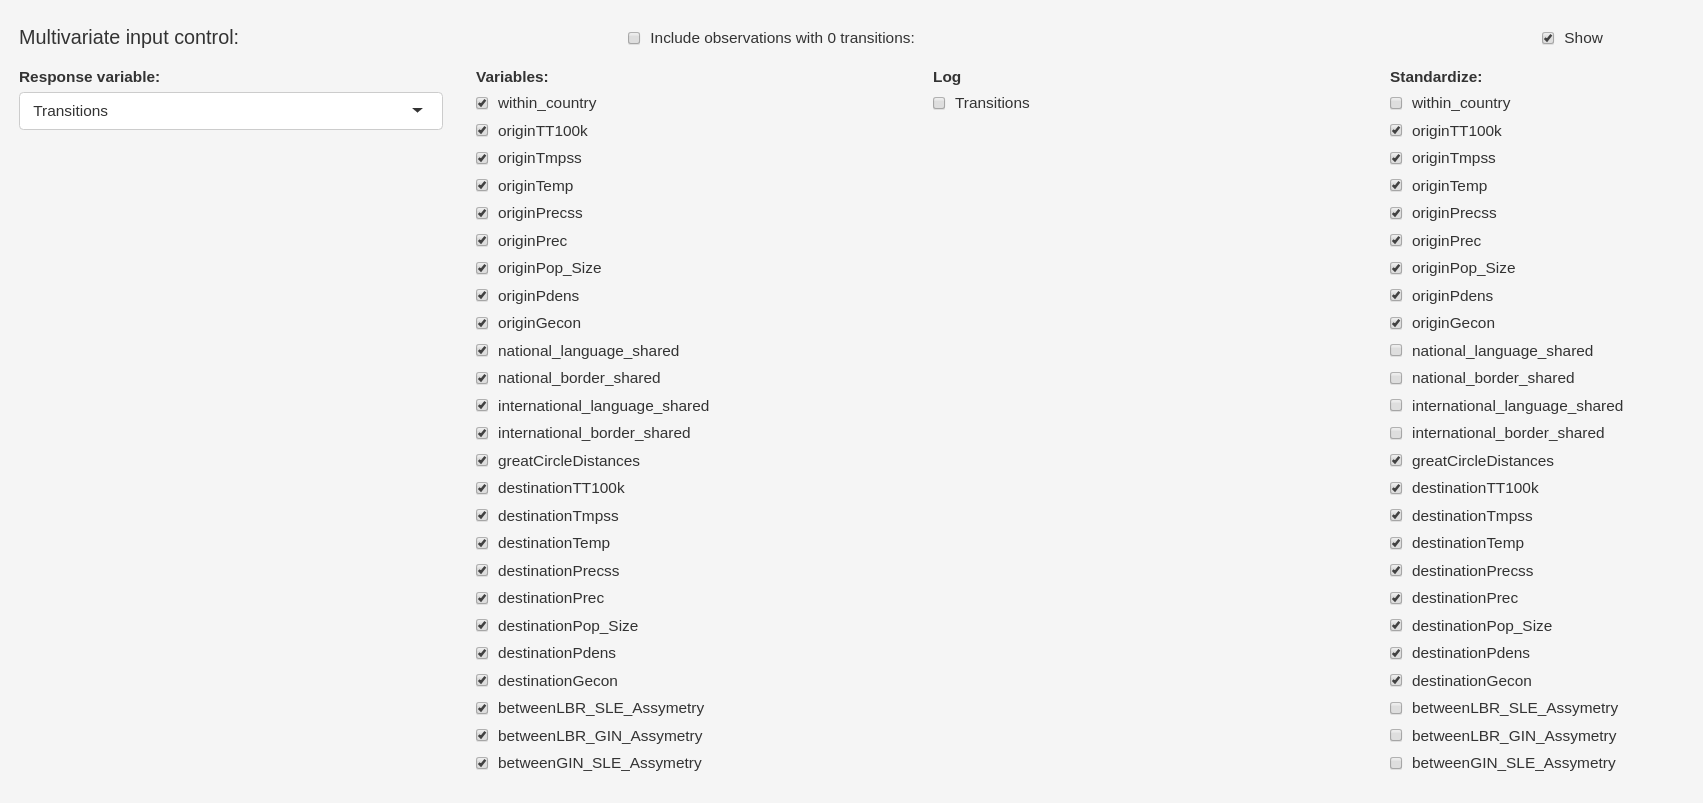
\includegraphics{tutorial_img/Variable_Selection.png}

We can hide this panel now and move to the regression output. It is
always a good idea to hide panels that are not needed. Anything not
displayed will not be computed and will speed up the analysis. This
effect is especially big when having many variables, including zero
transitions and having the plotting panel open. \textbf{Always hide the
plotting panel before changing variable selection}.

The summary output shows the type III sum of squares:

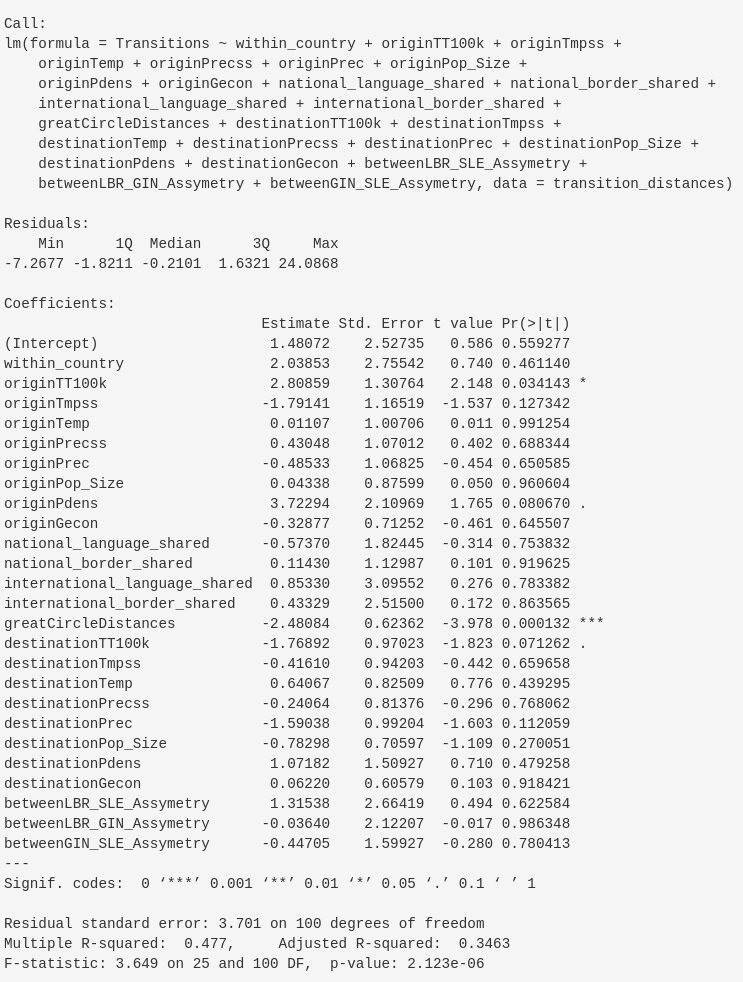
\includegraphics{tutorial_img/summary_multi.png}

Here, we can note an adjusted R² of 35\%, meaning that this model
explains 35\% of the variation in the transition counts after adjusting
for the number of predictors included in the model. We can now take a
look at the variable selection via the ``leaps'' package and the
``regsubsets'' function, which makes use of different criteria to select
the best model according to e.g.~``BIC'' out of all possible subsets of
variables or via the backward/forward selection.

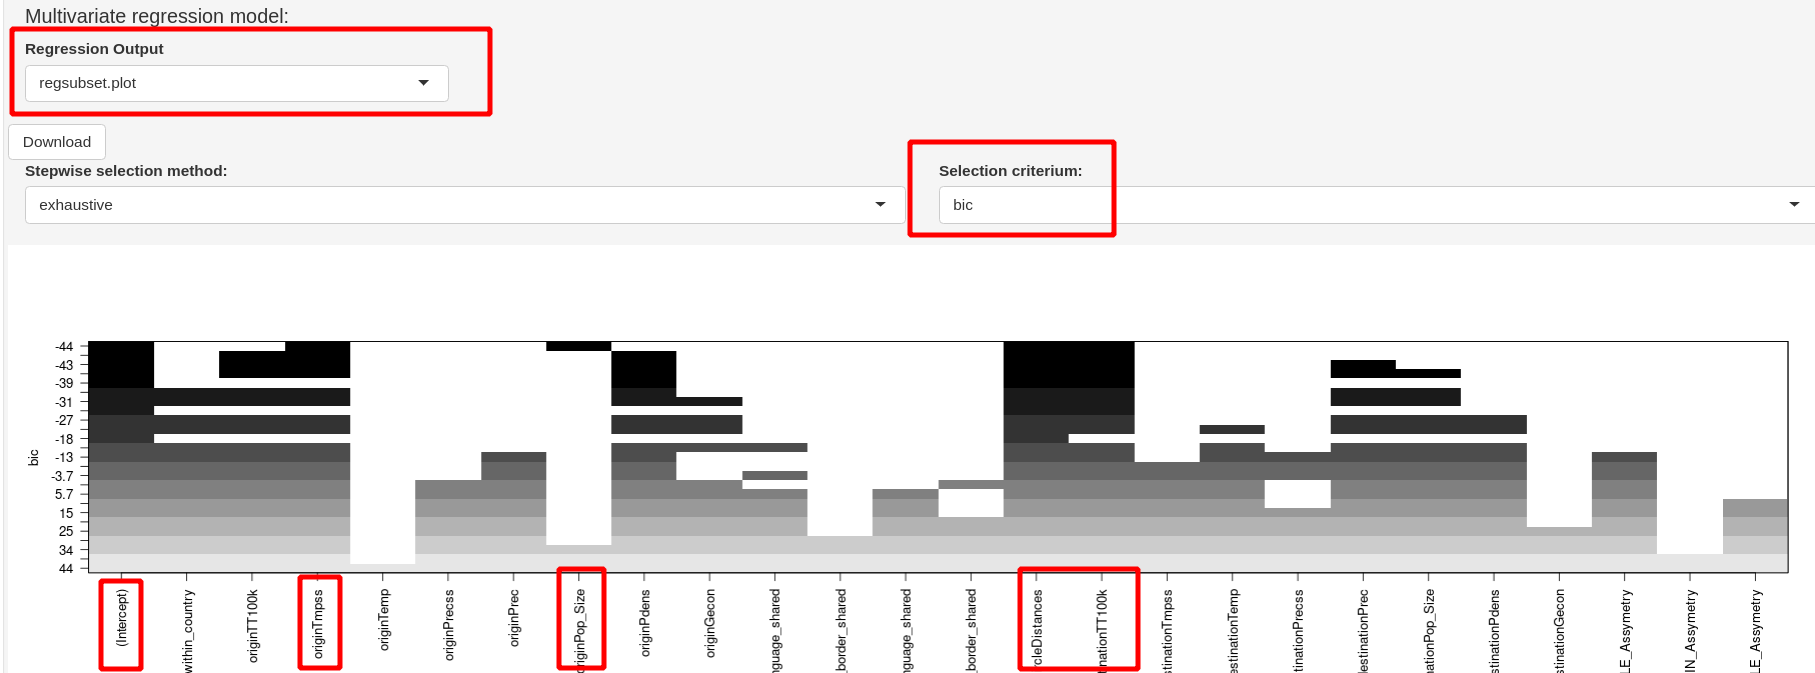
\includegraphics{tutorial_img/regsubsets.ong.png}

This plot shows 1 model for each number of variables. Each model is the
best model for this amount of variables according to the BIC criterion.
These pre-selected models are then sorted by their BIC value with the
lowest BIC value on top. So the best model overall is listed in the top
row. Blackened squares mean that the variable has been selected. We can
note that the best model is a 4-variable model consisting of: the
temperature at the origin location, the population size at the origin
location, the geographic distance and the travel distance to the next
metropolitan area from the destination location.

\textbf{Note:} For this data set using the backward selection algorithm
leads to a 5-variable model. This output will also be found in the
stepwise AIC model when using the ``BIC'' criterion.

We can now go ahead and build a linear model with only the seleced
variabeles:

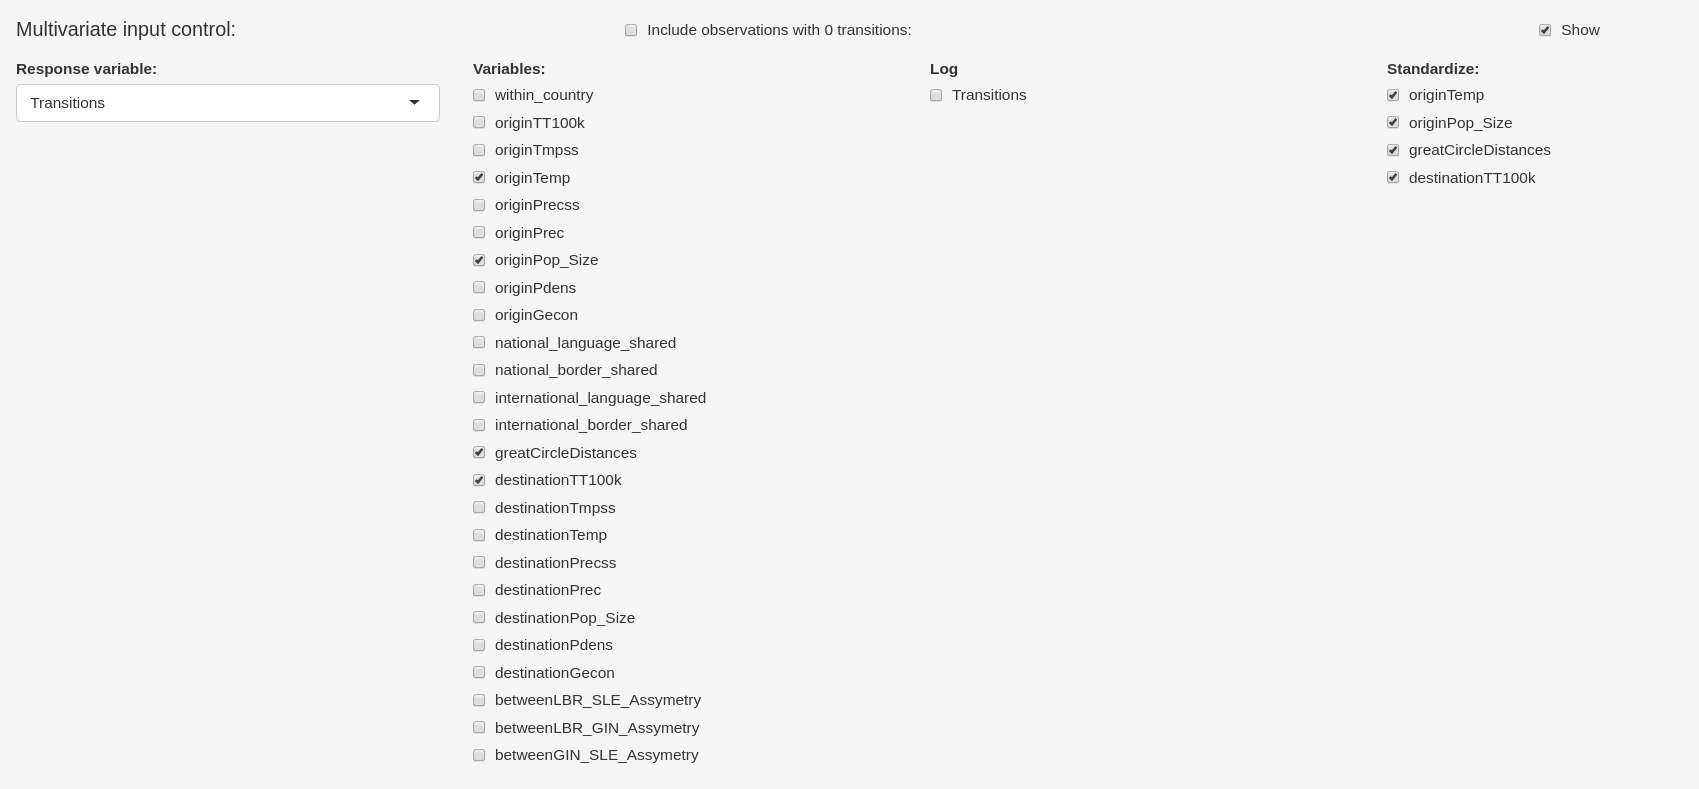
\includegraphics{tutorial_img/Variable_SelectionSelected.png}

The adjusted R² for this data set did not change when reducing the model
to the selected variables only.

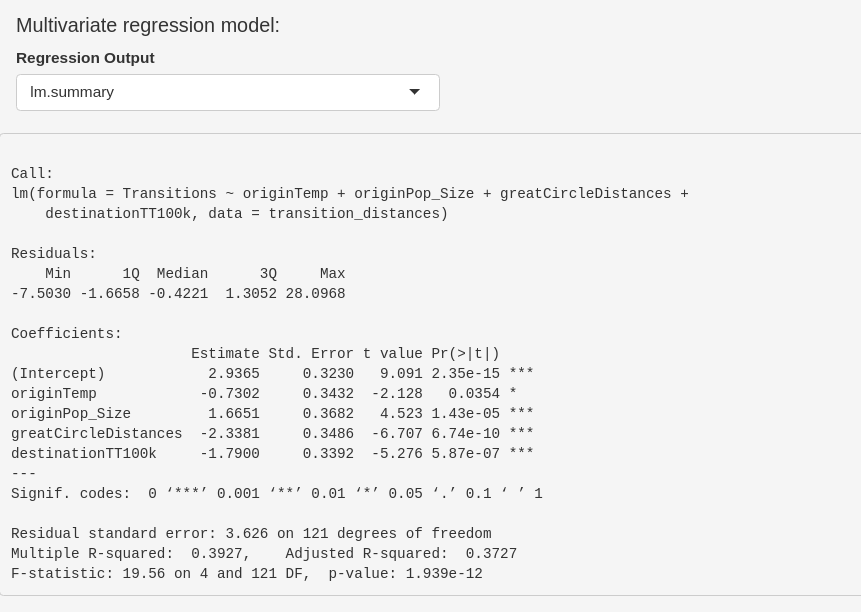
\includegraphics{tutorial_img/summary_multi_selected.png}

To conclude the Multivariate tab we can move on to the plotting panel:

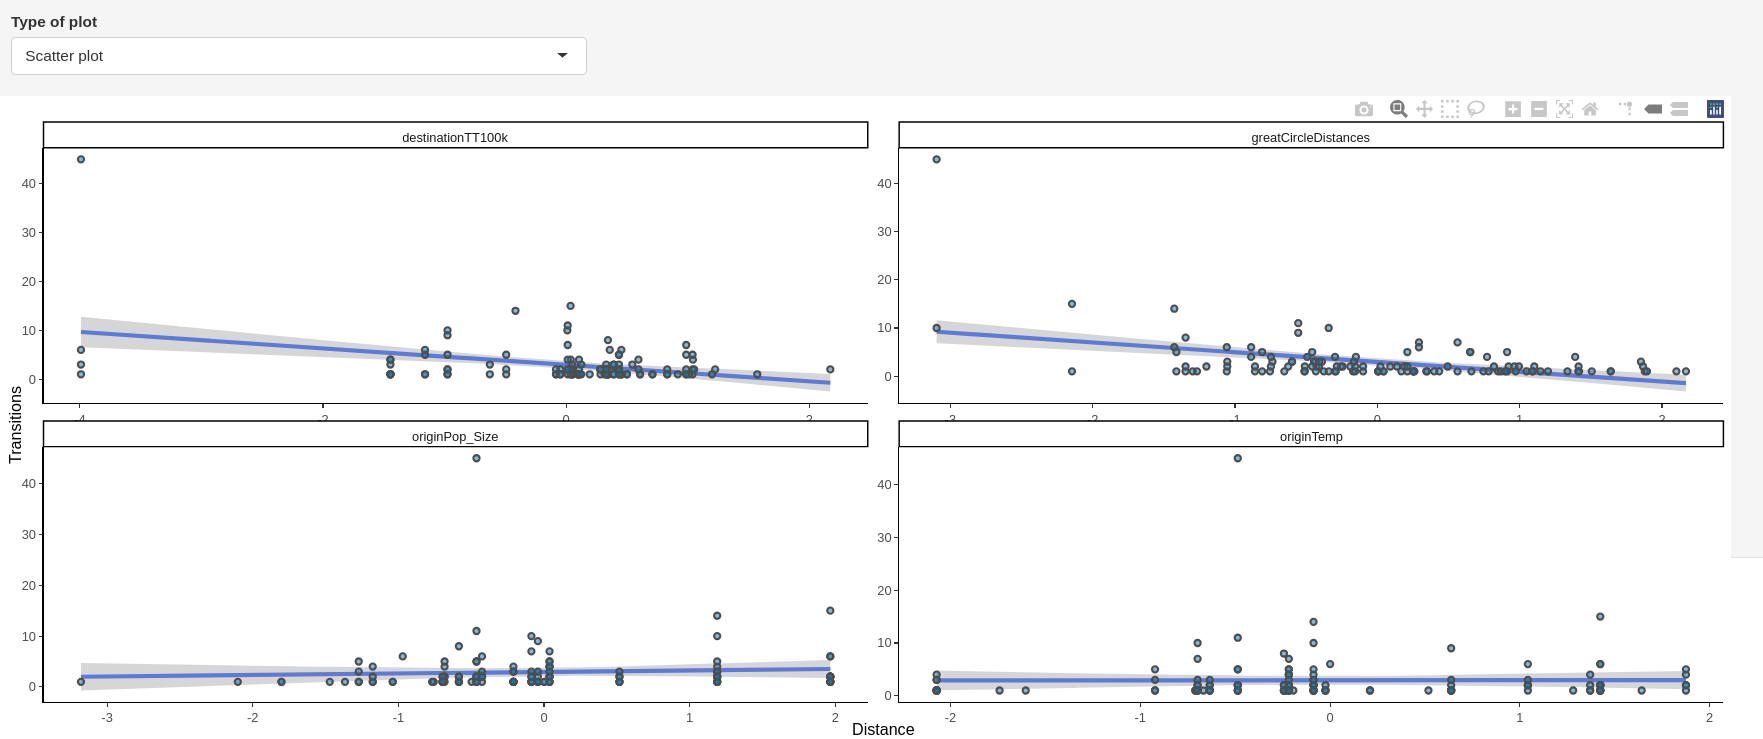
\includegraphics{tutorial_img/scatter_multi.png}

In addition correlation plots can be visualized:

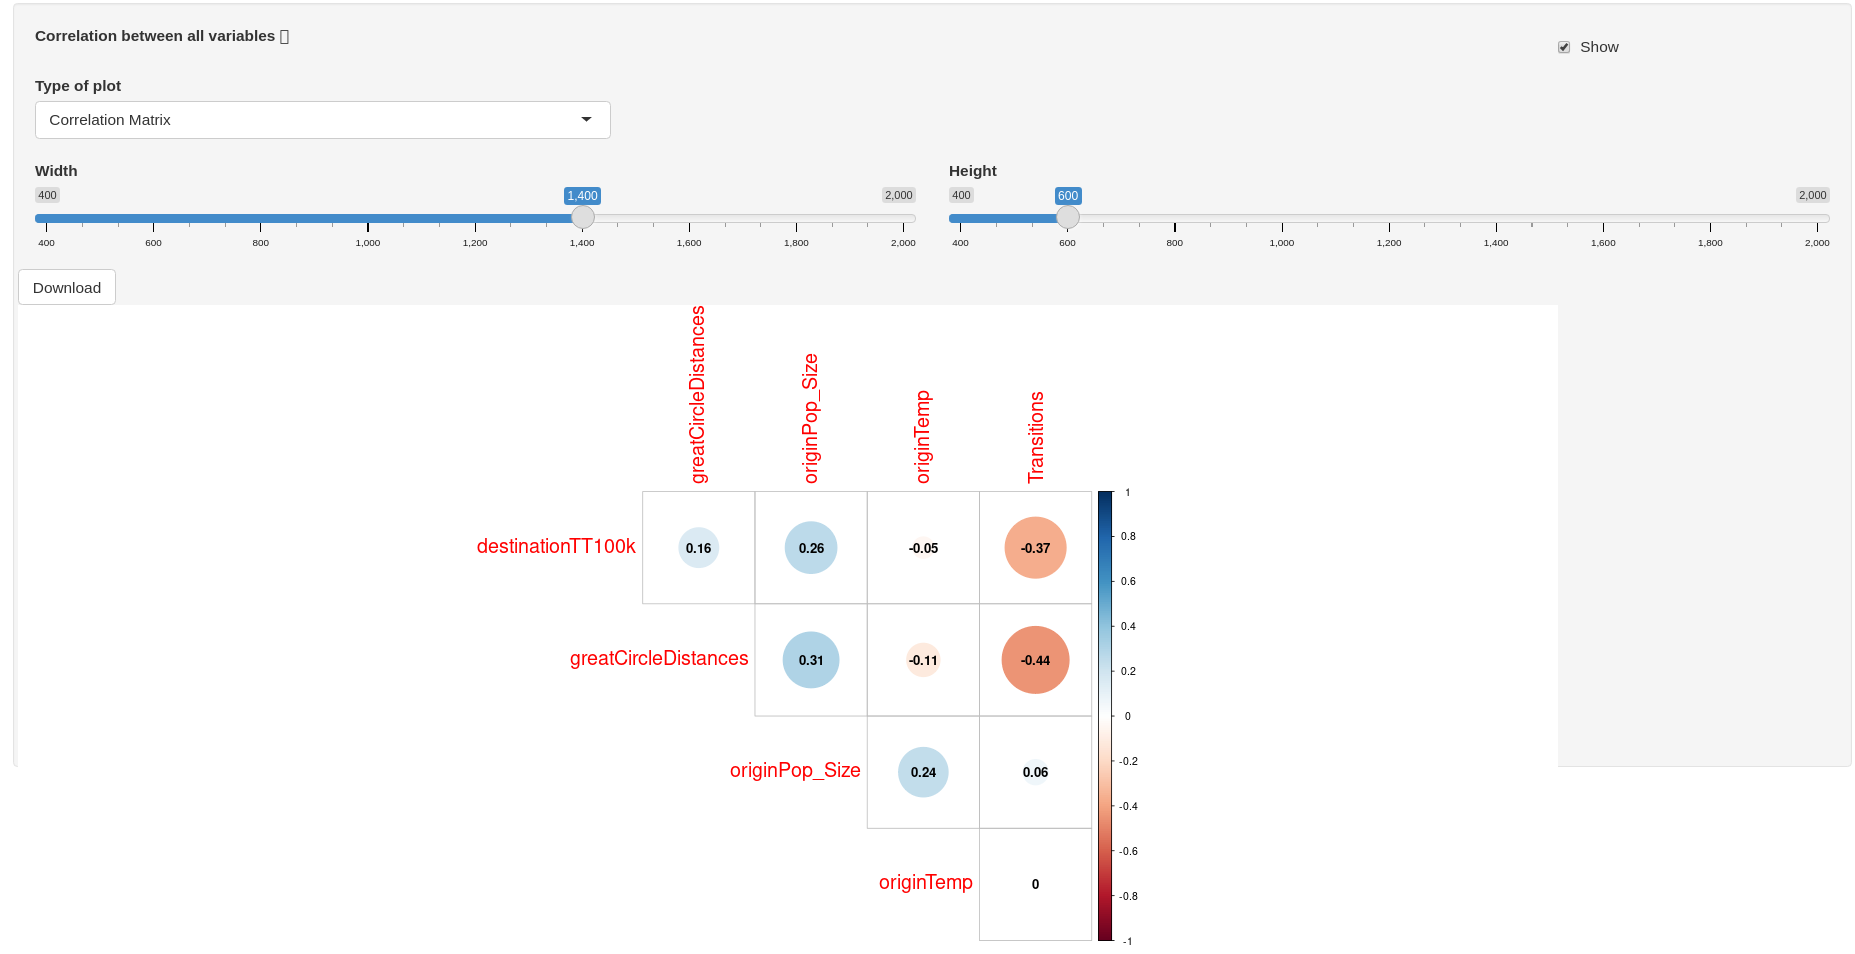
\includegraphics{tutorial_img/Corplotpng.png}

\hypertarget{tree-exploration}{%
\subsubsection{Tree exploration}\label{tree-exploration}}

The phylogeny can also be visualized in PhyCovA:

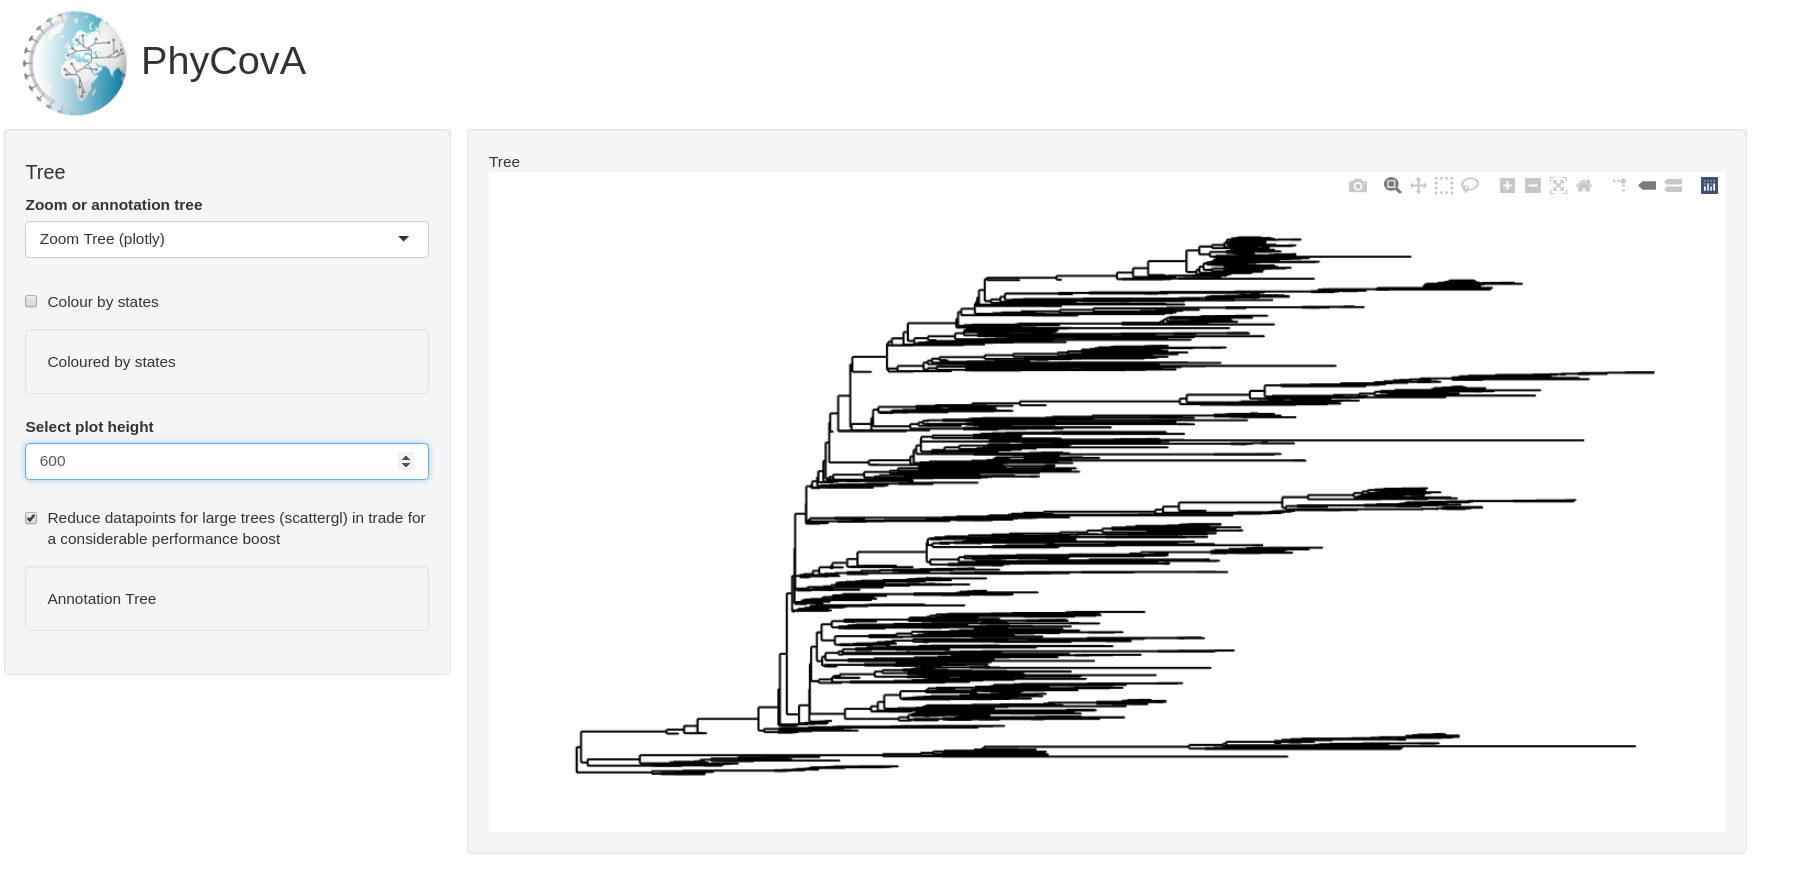
\includegraphics{tutorial_img/Tree_initial.png} This tree is generated
by ``Plotly'' and is zoomable, hence the name in the drop-down to the
right. The user has different tools available such as selection, panning
and zooming tools in the top right corner of the plotting area. The tree
height can also be changed and very large plots can be plotted and one
can scroll through the plot. One can also colour the tree and show more
of the availale information by ticking the box for ``Coloured by
states'' and unticking the box for ``Reduce datapoints for large trees
(scattergl) in trade for a condirate performance boost''.

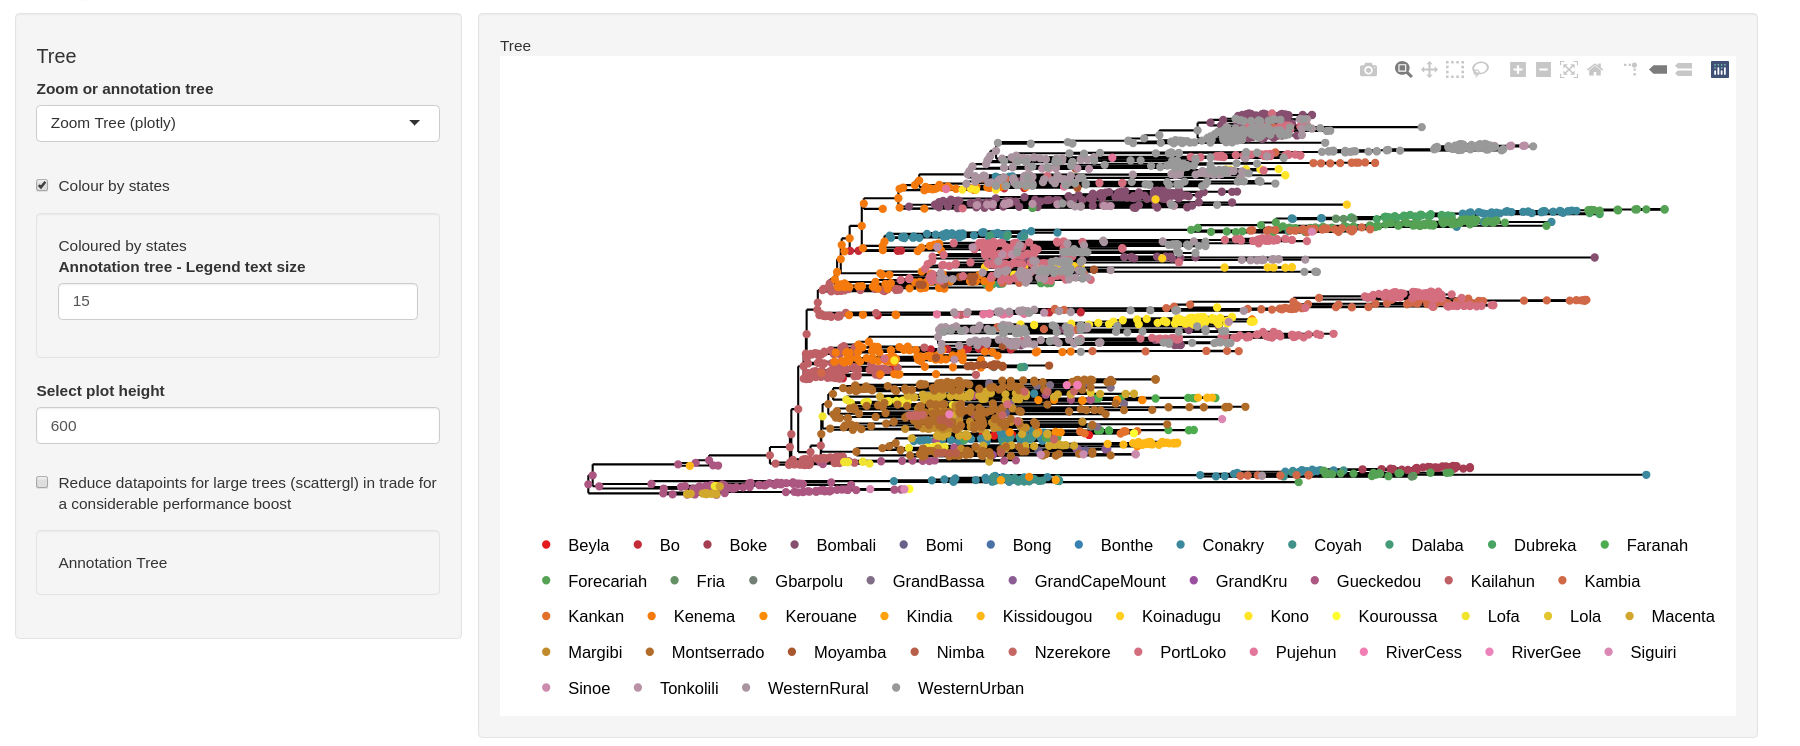
\includegraphics{tutorial_img/coloured_tree.png}

Unticking the latter box is only affecting information in the tooltips.

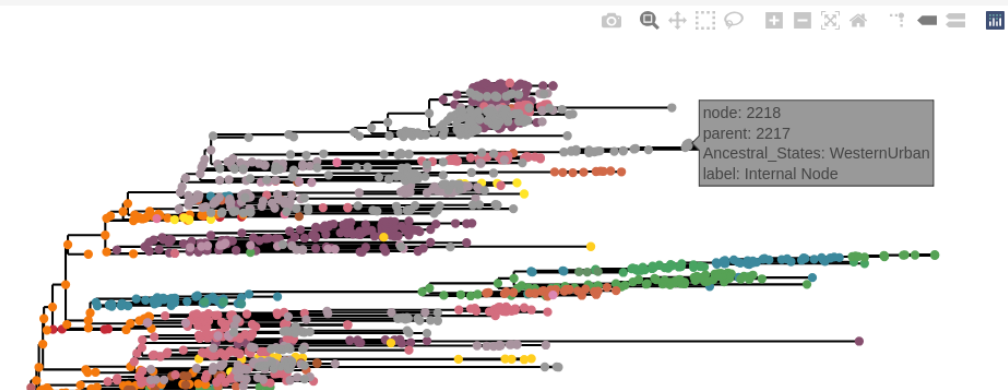
\includegraphics{tutorial_img/tooltip.png}

One can only highlight only certain states, to see where this state is
located in the tree. This is here done by double-clikcing on the state
in the legend. We can see that Gueckedou was the likely starting point
of the Ebola pandemic as it is mainly annotated as state at the root and
nodes in proximity of the root of the phylogeny.

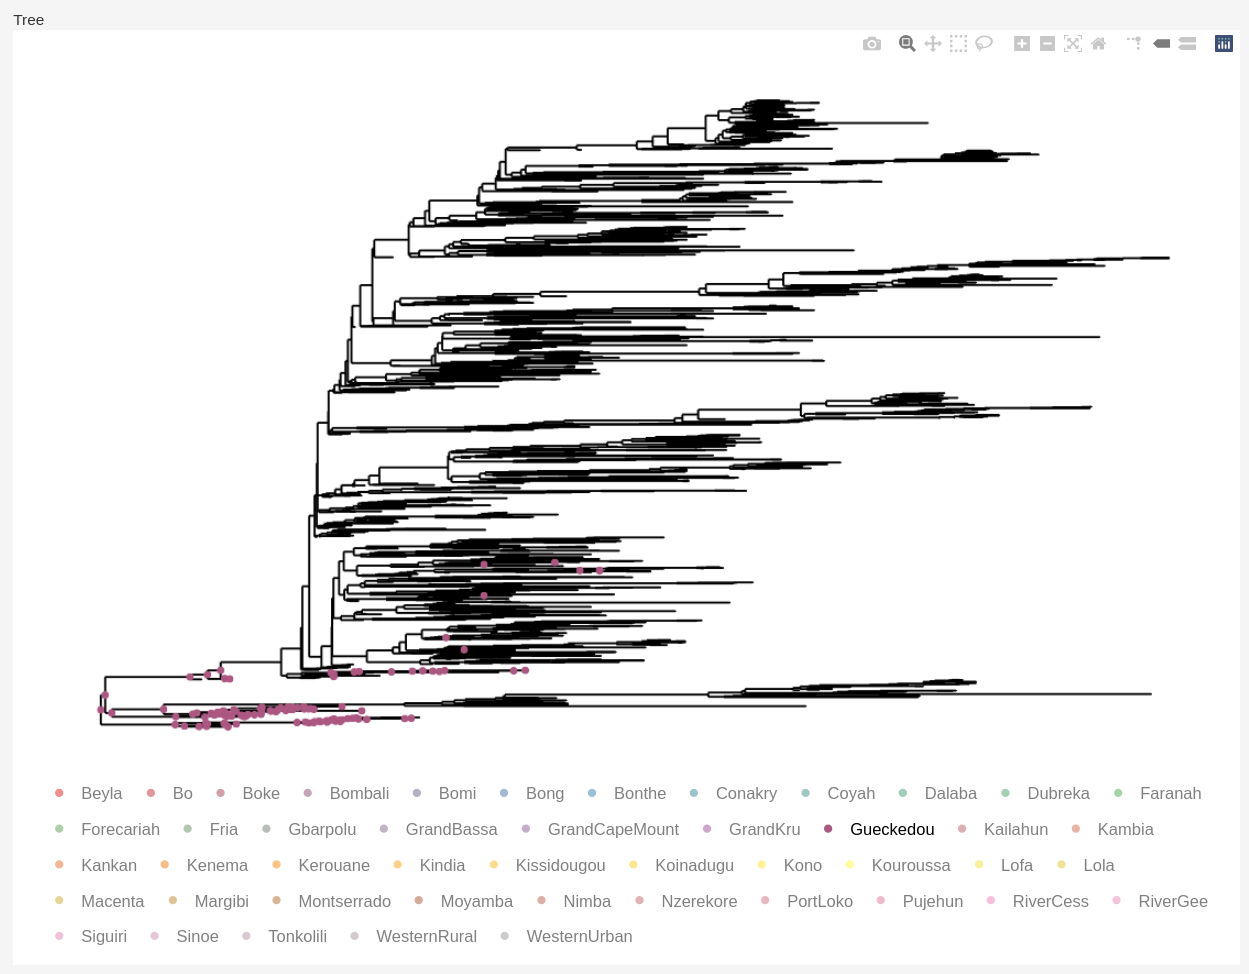
\includegraphics{tutorial_img/Gueckedou.png}

Next to a zoomable tree there is also a non-zoomable tree, which can be
annotated in more detail. The 2 trees are intended to work together. One
possible use case is to identify the region of a tree of interest. Get
the node number of the tree via the tooltip, e.g.~in this example above
this was node 2218. We can look at only this node and its offspring in
the annotation tree:

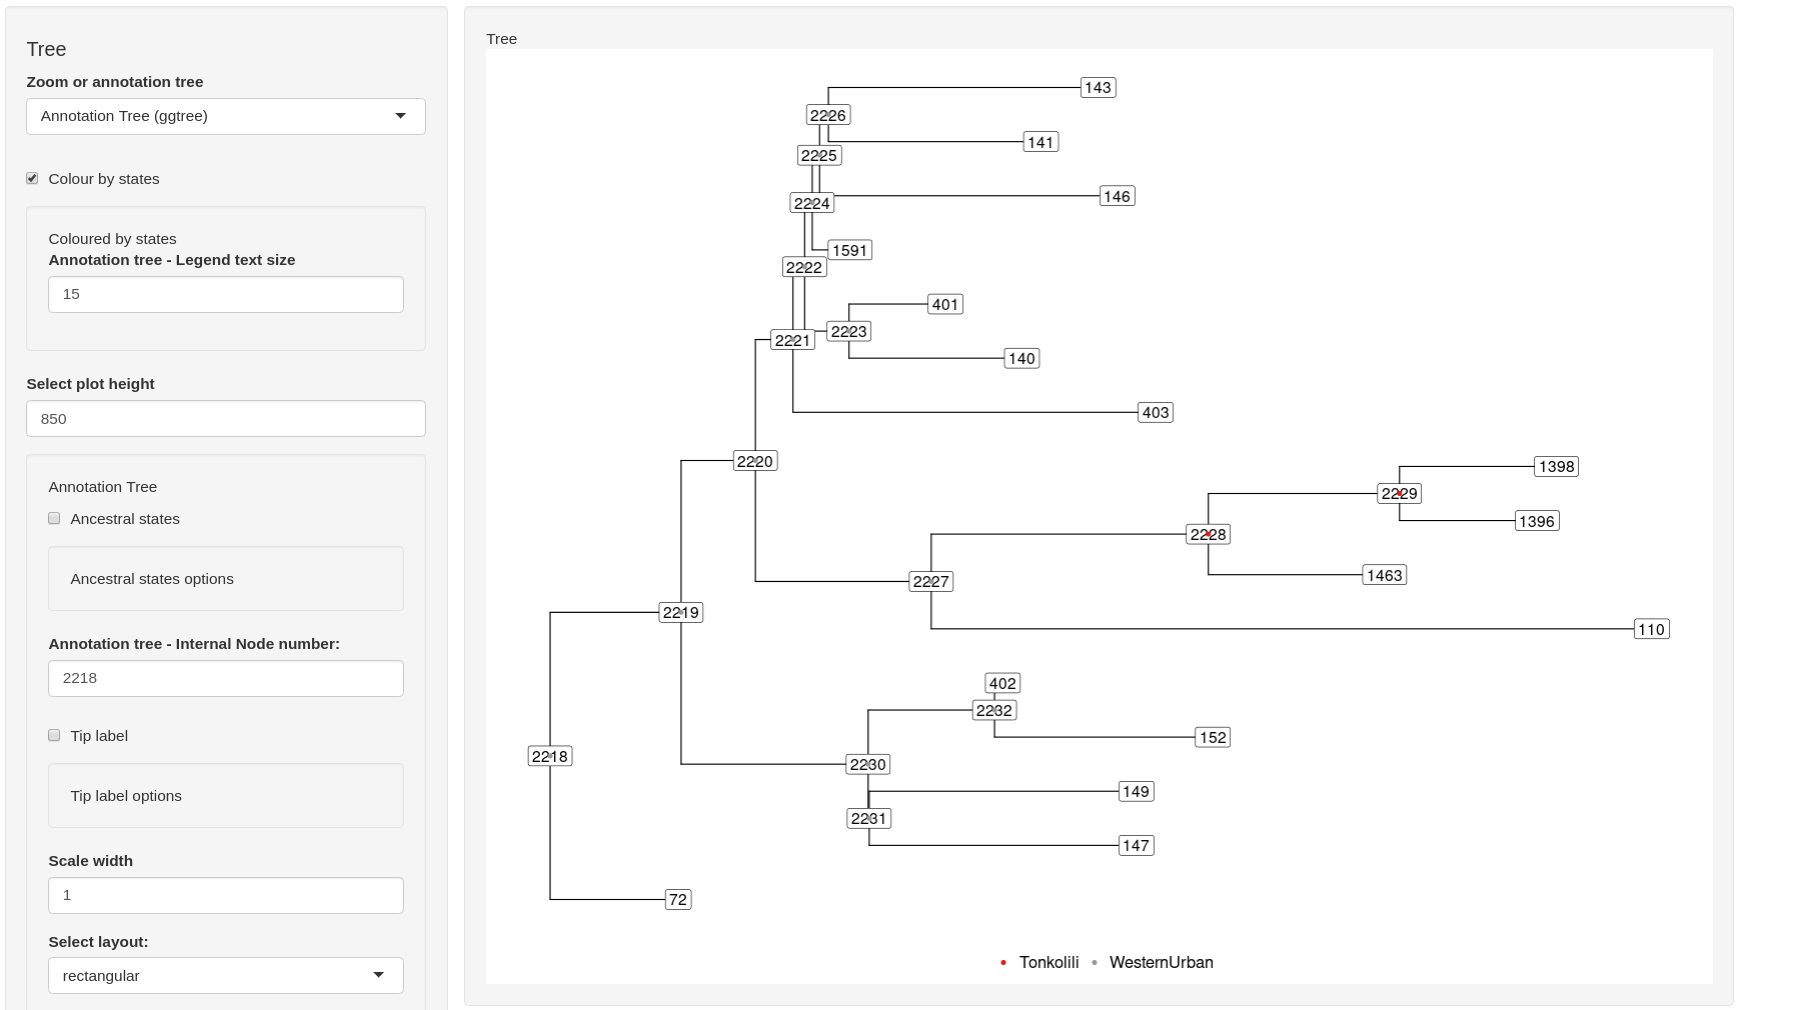
\includegraphics{tutorial_img/nodenumber.png}

And from this subtree many annotations can be shown on the tree, like
the ancestral state, the node shapes etc.

\hypertarget{reset}{%
\subsection{Reset}\label{reset}}

In case one has finished analyzing the data set and wants to analyze
something else, one opens the ``Univariate'' tab and clicks ``RESET''.
Now all input is cleared and new files can be uploaded.

\hypertarget{non-annotated-tree}{%
\subsection{Non-Annotated tree}\label{non-annotated-tree}}

For non-annotated trees, also a phylogeny and at least 1 distance matrix
is required. In addition to these 2 files PhyCovA required a sorted list
of tip states and the states need be \textbf{exactly} the same as the
column names in the distance matrices.

One can now select 1 of the 3 possible reconstruction methods and carry
out the analysis as described above for the annotated case.

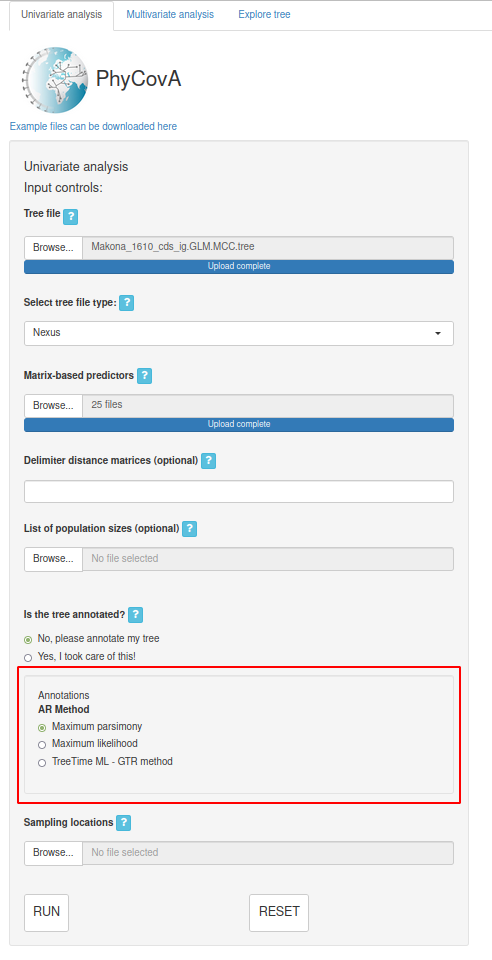
\includegraphics{tutorial_img/Non_annotated.png}

This concludes the tutorial for PhyCovA.

\end{document}
